% Sources of disagreement between SCDC, BayesPrism and DWLS when each
% method builds its own signature from one reference: composite for
% docs/04-deconvolution-pipeline.qmd, #fig-kappa-gastruloid (Scenario 1,
% #sec-deconv-own-genes). Replaces the AI-drawn
% images/condition_number_poor_performance_correlated_cell_types.png.
%
% A: shared notation (bayesnet model) and the example lineage continuum.
% B: how each method builds its reference. C: inference step, and the
% hypothesis of the chapter. Every rule drawn here is stated in the
% chapter text and in #tbl-deconv-own-genes; the figure carries no result.
%
% Build (from this directory):
%   lualatex -interaction=nonstopmode -halt-on-error kappa_gastruloid.tex
%   gs -q -dNOPAUSE -dBATCH -dNoOutputFonts -sDEVICE=pdfwrite \
%     -o ../../fig_04_kappa_gastruloid.pdf kappa_gastruloid.pdf
%   pdftocairo -svg ../../fig_04_kappa_gastruloid.pdf ../../fig_04_kappa_gastruloid.svg
% Then delete any white page rectangle that pdftocairo adds to the SVG,
% check that `pdffonts ../../fig_04_kappa_gastruloid.pdf` lists no font,
% and remove the LaTeX build products (aux, log, pdf) from this directory.
\documentclass[tikz,border=4pt]{standalone}
\usepackage{iftex}
\ifPDFTeX
  \PackageError{kappa_gastruloid}{Use LuaLaTeX or XeLaTeX}{}
\fi
\usepackage{amsmath}
\usepackage{fontspec}
\usepackage{unicode-math}
\setmathfont{STIX Two Math}
\setmainfont{TeX Gyre Heros}[Ligatures=CommonOff]
\usetikzlibrary{bayesnet,positioning,fit,calc,arrows.meta,backgrounds,shapes.geometric}
% palette of docs/_quarto.yml; one accent per method header
\definecolor{ink}{HTML}{1F2937}
\definecolor{latfill}{HTML}{DAE9FB}
\definecolor{latdraw}{HTML}{4477B5}
\definecolor{obsfill}{HTML}{C9CDD3}
\definecolor{obsdraw}{HTML}{747B86}
\definecolor{accscdc}{HTML}{2E7D6B}
\definecolor{accbp}{HTML}{6A4C93}
\definecolor{accdwls}{HTML}{C45C26}
\tikzset{
  every node/.style={text=ink},
  fixed/.style={const, draw, minimum size=7mm, inner sep=2pt},
  note/.style={font=\footnotesize, align=left},
  dependency/.style={-{Stealth[length=2mm]}, semithick, draw=ink},
  panel/.style={draw=obsdraw, rounded corners=4pt, line width=0.6pt},
  tag/.style={font=\bfseries\large, anchor=north west, inner sep=0pt},
  ptitle/.style={font=\bfseries\small, anchor=west, inner sep=0pt},
  colbox/.style={draw=obsdraw!70, rounded corners=3pt, line width=0.5pt},
  colhead/.style={font=\bfseries\small, anchor=north west, inner sep=0pt},
  colsub/.style={font=\footnotesize\itshape, anchor=north west, inner sep=0pt, text=ink!80},
  bullets/.style={note, anchor=north west, text width=#1, inner sep=0pt},
  state/.style={rectangle, rounded corners=3pt, draw=obsdraw, fill=obsfill!45,
    line width=0.6pt, font=\footnotesize, inner sep=1.6mm, minimum height=6mm},
  flow/.style={-{Stealth[length=2mm]}, semithick, draw=ink},
  hyp/.style={draw=ink, dashed, rounded corners=3pt, line width=0.6pt,
    fill=obsfill!20, note, text width=#1, inner sep=2.2mm}
}
\newcommand{\bitem}[1]{\par\noindent\makebox[0.9em][l]{\textbullet}\parbox[t]{\dimexpr\hsize-0.9em\relax}{\raggedright #1}}
% \methodcol{x left}{y top}{width}{height}{colour}{name}{subtitle}
\newcommand{\methodcol}[7]{%
  \draw[colbox] (#1,#2) rectangle ++(#3,-#4);
  \fill[#5] (#1,#2) ++(0.25,-0.22) rectangle ++(0.12,-0.62);
  \node[colhead, text=#5] at ($(#1,#2)+(0.5,-0.2)$) {#6};
  \node[colsub] at ($(#1,#2)+(0.5,-0.58)$) {#7};
}
\begin{document}
\hyphenpenalty=10000
\exhyphenpenalty=10000
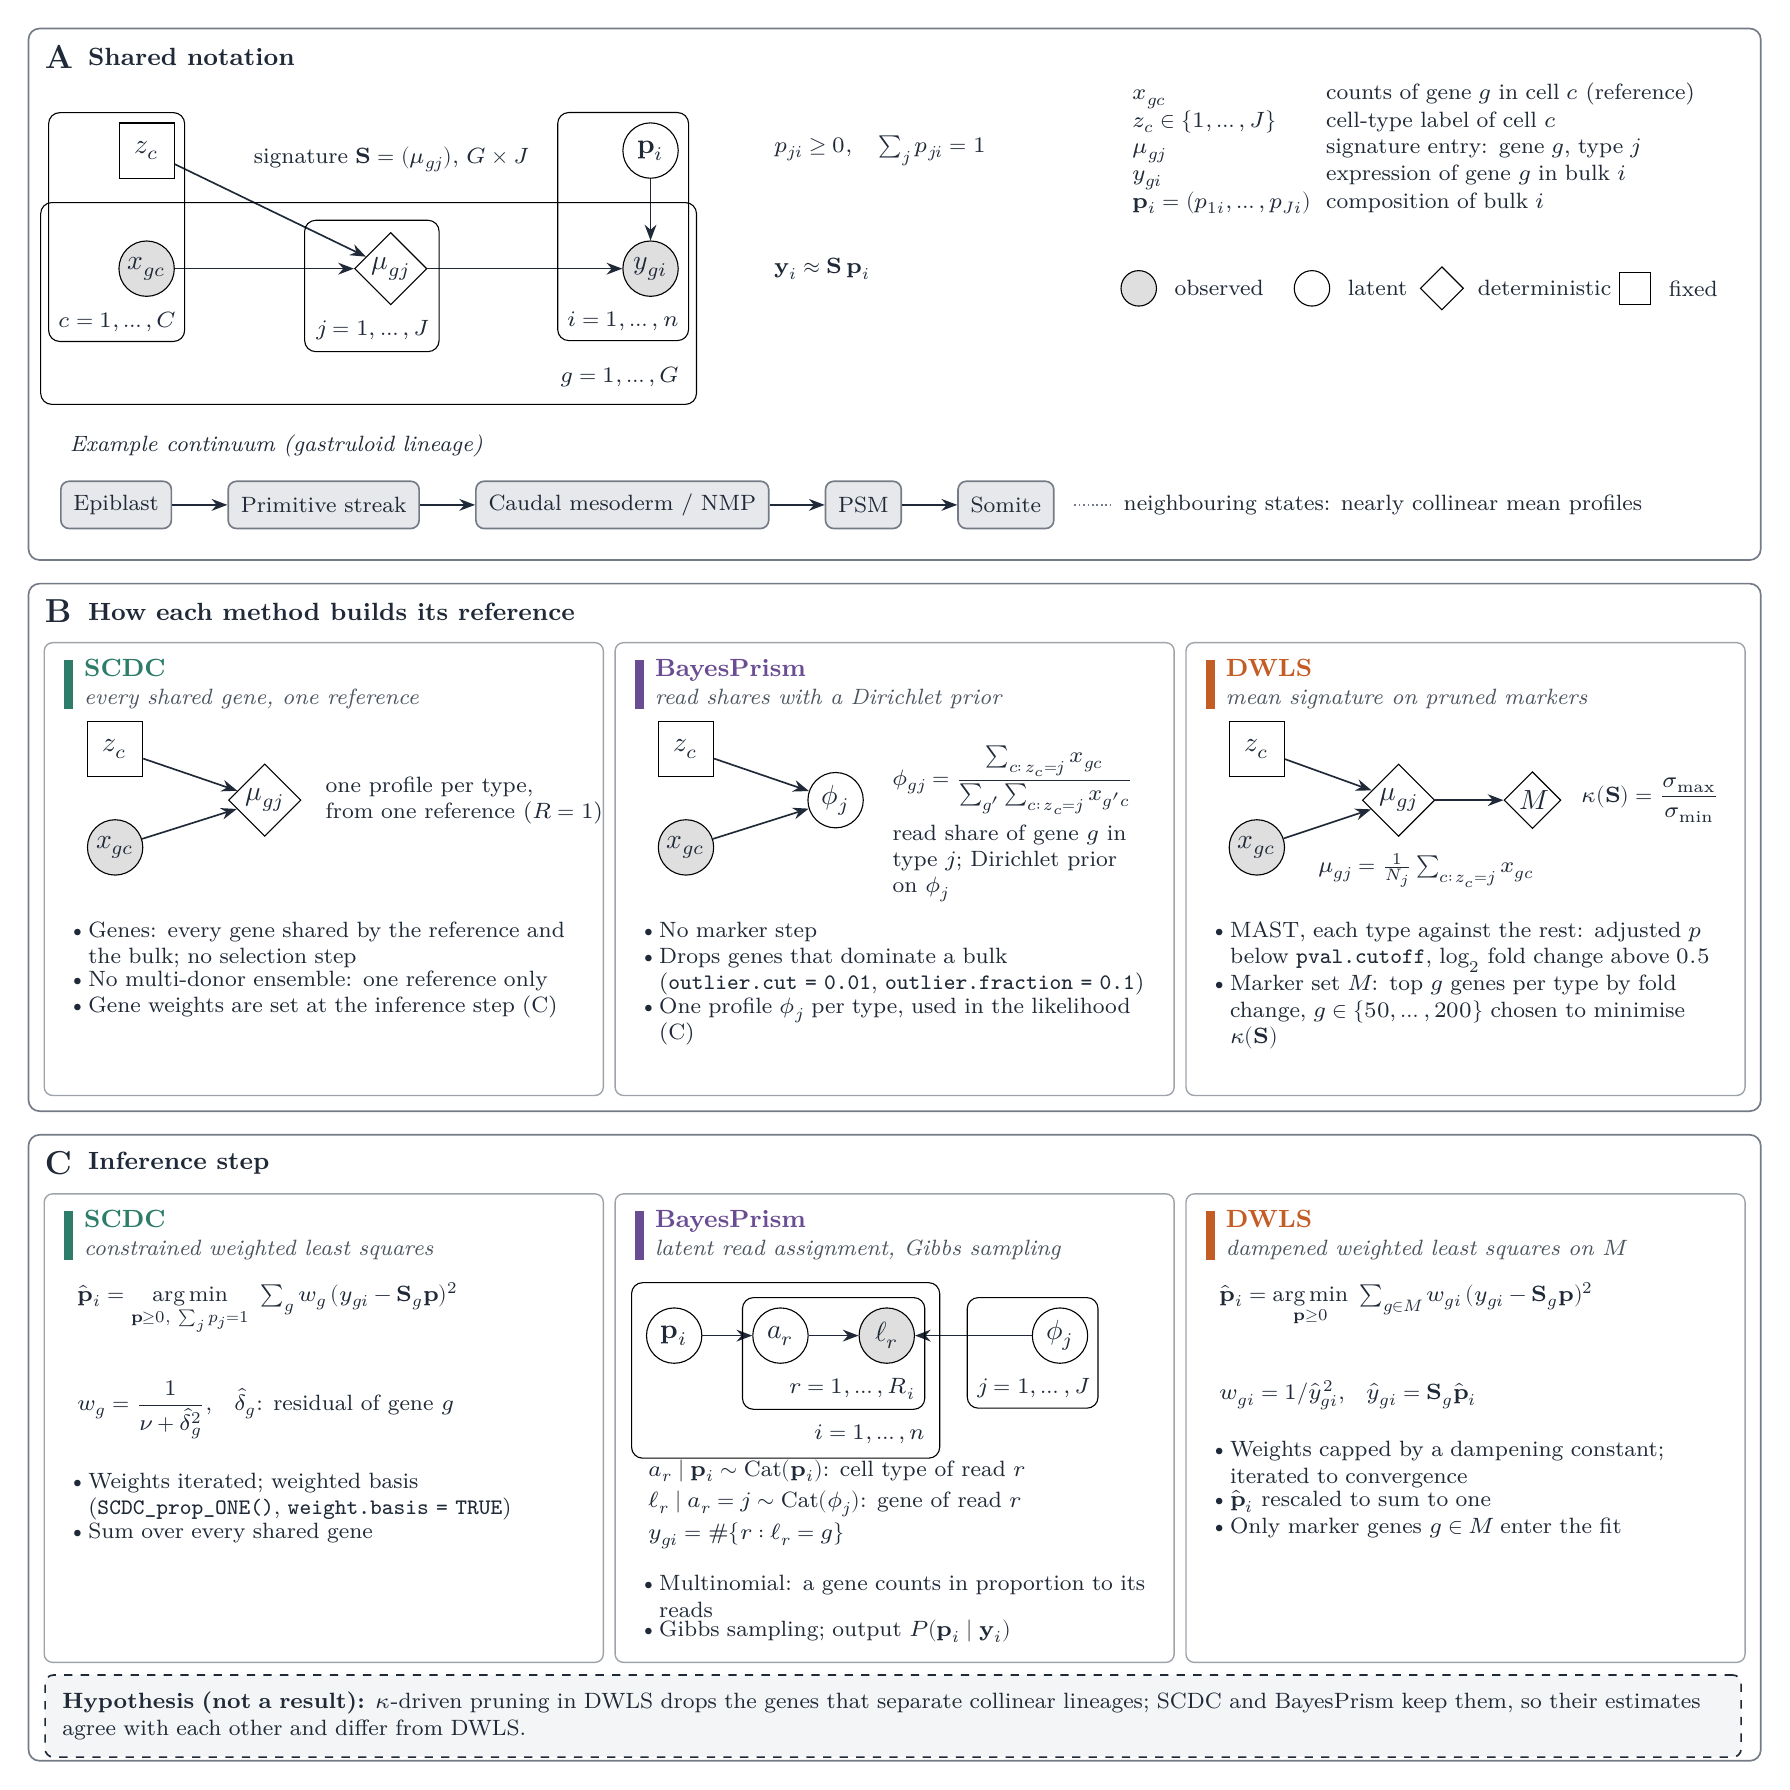
\begin{tikzpicture}
% ---------------------------------------------------------------- A
\draw[panel] (0,0) rectangle (22,-6.75);
\node[tag] at (0.2,-0.2) {A};
\node[ptitle] at (0.75,-0.36) {Shared notation};
% model: single-cell reference, signature, bulk
\node[fixed] (zA) at (1.5,-1.55) {$z_c$};
\node[obs]   (xA) at (1.5,-3.05) {$x_{gc}$};
\node[det]   (muA) at (4.6,-3.05) {$\mu_{gj}$};
\node[latent] (pA) at (7.9,-1.55) {$\symbf{p}_i$};
\node[obs]   (yA) at (7.9,-3.05) {$y_{gi}$};
\draw[dependency] (xA) -- (muA);
\draw[dependency] (zA) -- (muA);
\draw[dependency] (muA) -- (yA);
\draw[dependency] (pA) -- (yA);
\plate[inner sep=4pt]{plJ}{(muA)}{$j=1,\dots,J$}
\plate{plC}{(zA)(xA)}{$c=1,\dots,C$}
\plate{plI}{(pA)(yA)}{$i=1,\dots,n$}
\plate[inner sep=6pt]{plG}{(xA)(muA)(yA)(plJ)(plC-caption)(plI-caption)}{$g=1,\dots,G$}
\node[note, anchor=south] at (4.6,-1.95) {signature $\symbf{S}=(\mu_{gj})$, $G\times J$};
\node[note, anchor=west] at (9.35,-1.55) {$p_{ji}\ge 0,\quad \sum_{j} p_{ji}=1$};
\node[note, anchor=west] at (9.35,-3.05) {$\symbf{y}_i\approx\symbf{S}\,\symbf{p}_i$};
% key to symbols and node shapes
\node[note, anchor=north west, text width=7.6cm] at (13.9,-0.55) {%
  \begin{tabular}{@{}l@{\ \ }l@{}}
  $x_{gc}$ & counts of gene $g$ in cell $c$ (reference)\\
  $z_c\in\{1,\dots,J\}$ & cell-type label of cell $c$\\
  $\mu_{gj}$ & signature entry: gene $g$, type $j$\\
  $y_{gi}$ & expression of gene $g$ in bulk $i$\\
  $\symbf{p}_i=(p_{1i},\dots,p_{Ji})$ & composition of bulk $i$
  \end{tabular}};
\begin{scope}[shift={(14.1,-3.3)}]
  \node[obs, minimum size=4.5mm] (k1) at (0,0) {};
  \node[note, right=1mm of k1] {observed};
  \node[latent, minimum size=4.5mm] (k2) at (2.2,0) {};
  \node[note, right=1mm of k2] {latent};
  \node[det, minimum size=5.5mm] (k3) at (3.85,0) {};
  \node[note, right=0.5mm of k3] {deterministic};
  \node[fixed, minimum size=4mm] (k4) at (6.3,0) {};
  \node[note, right=1mm of k4] {fixed};
\end{scope}
% example continuum
\node[note, anchor=west, font=\footnotesize\itshape] at (0.4,-5.3)
  {Example continuum (gastruloid lineage)};
\node[state, anchor=west] (s1) at (0.4,-6.05) {Epiblast};
\node[state, right=7mm of s1] (s2) {Primitive streak};
\node[state, right=7mm of s2] (s3) {Caudal mesoderm / NMP};
\node[state, right=7mm of s3] (s4) {PSM};
\node[state, right=7mm of s4] (s5) {Somite};
\foreach \a/\b in {s1/s2, s2/s3, s3/s4, s4/s5} \draw[flow] (\a) -- (\b);
\draw[obsdraw, densely dotted, semithick] ($(s5.east)+(0.25,0)$) -- ++(0.5,0)
  node[note, anchor=west, text=ink] {neighbouring states: nearly collinear mean profiles};
% ---------------------------------------------------------------- B
\begin{scope}[shift={(0,-7.05)}]
\draw[panel] (0,0) rectangle (22,-6.7);
\node[tag] at (0.2,-0.2) {B};
\node[ptitle] at (0.75,-0.36) {How each method builds its reference};
\methodcol{0.2}{-0.75}{7.1}{5.75}{accscdc}{SCDC}{every shared gene, one reference}
\methodcol{7.45}{-0.75}{7.1}{5.75}{accbp}{BayesPrism}{read shares with a Dirichlet prior}
\methodcol{14.7}{-0.75}{7.1}{5.75}{accdwls}{DWLS}{mean signature on pruned markers}
% SCDC
\node[fixed] (zB1) at (1.1,-2.10) {$z_c$};
\node[obs]   (xB1) at (1.1,-3.35) {$x_{gc}$};
\node[det]   (muB1) at (3.0,-2.75) {$\mu_{gj}$};
\draw[dependency] (zB1) -- (muB1);
\draw[dependency] (xB1) -- (muB1);
\node[note, anchor=west] at (3.65,-2.75) {one profile per type,\\from one reference ($R=1$)};
\node[bullets=6.6cm] at (0.5,-4.15) {%
  \bitem{Genes: every gene shared by the reference and the bulk; no selection step}
  \bitem{No multi-donor ensemble: one reference only}
  \bitem{Gene weights are set at the inference step (C)}};
% BayesPrism
\node[fixed] (zB2) at (8.35,-2.10) {$z_c$};
\node[obs]   (xB2) at (8.35,-3.35) {$x_{gc}$};
\node[latent] (phB2) at (10.25,-2.75) {$\phi_j$};
\draw[dependency] (zB2) -- (phB2);
\draw[dependency] (xB2) -- (phB2);
\node[note, anchor=west] at (10.85,-2.50)
  {$\phi_{gj}=\dfrac{\sum_{c:\,z_c=j}x_{gc}}{\sum_{g'}\sum_{c:\,z_c=j}x_{g'c}}$};
\node[note, anchor=west] at (10.85,-3.55) {read share of gene $g$ in\\type $j$; Dirichlet prior\\on $\phi_j$};
\node[bullets=6.6cm] at (7.75,-4.15) {%
  \bitem{No marker step}
  \bitem{Drops genes that dominate a bulk (\mbox{\texttt{outlier.cut = 0.01}}, \mbox{\texttt{outlier.fraction = 0.1}})}
  \bitem{One profile $\phi_j$ per type, used in the likelihood (C)}};
% DWLS
\node[fixed] (zB3) at (15.6,-2.10) {$z_c$};
\node[obs]   (xB3) at (15.6,-3.35) {$x_{gc}$};
\node[det]   (muB3) at (17.4,-2.75) {$\mu_{gj}$};
\node[det]   (MB3) at (19.1,-2.75) {$M$};
\draw[dependency] (zB3) -- (muB3);
\draw[dependency] (xB3) -- (muB3);
\draw[dependency] (muB3) -- (MB3);
\node[note, anchor=north] at (17.75,-3.30) {$\mu_{gj}=\frac{1}{N_j}\sum_{c:\,z_c=j}x_{gc}$};
\node[note, anchor=west] at (19.6,-2.75) {$\kappa(\symbf{S})=\dfrac{\sigma_{\max}}{\sigma_{\min}}$};
\node[bullets=6.7cm] at (15.0,-4.15) {%
  \bitem{MAST, each type against the rest: adjusted $p$ below \texttt{pval.cutoff}, $\log_2$ fold change above $0.5$}
  \bitem{Marker set $M$: top $g$ genes per type by fold change, $g\in\{50,\dots,200\}$ chosen to minimise $\kappa(\symbf{S})$}};
\end{scope}
% ---------------------------------------------------------------- C
\begin{scope}[shift={(0,-14.05)}]
\draw[panel] (0,0) rectangle (22,-7.95);
\node[tag] at (0.2,-0.2) {C};
\node[ptitle] at (0.75,-0.36) {Inference step};
\methodcol{0.2}{-0.75}{7.1}{5.95}{accscdc}{SCDC}{constrained weighted least squares}
\methodcol{7.45}{-0.75}{7.1}{5.95}{accbp}{BayesPrism}{latent read assignment, Gibbs sampling}
\methodcol{14.7}{-0.75}{7.1}{5.95}{accdwls}{DWLS}{dampened weighted least squares on $M$}
% SCDC
\node[note, anchor=north west] at (0.5,-1.75)
  {$\hat{\symbf{p}}_i=\underset{\symbf{p}\ge 0,\ \sum_j p_j=1}{\arg\min}\ \sum_{g} w_g\,(y_{gi}-\symbf{S}_g\symbf{p})^2$};
\node[note, anchor=north west] at (0.5,-3.0)
  {$w_g=\dfrac{1}{\nu+\hat\delta_g^{2}}$,\quad $\hat\delta_g$: residual of gene $g$};
\node[bullets=6.6cm] at (0.5,-4.15) {%
  \bitem{Weights iterated; weighted basis (\texttt{SCDC\_prop\_ONE()}, \mbox{\texttt{weight.basis = TRUE}})}
  \bitem{Sum over every shared gene}};
% BayesPrism
\node[latent] (pC) at (8.2,-2.55) {$\symbf{p}_i$};
\node[latent] (aC) at (9.55,-2.55) {$a_r$};
\node[obs]    (lC) at (10.9,-2.55) {$\ell_r$};
\node[latent] (phC) at (13.1,-2.55) {$\phi_j$};
\draw[dependency] (pC) -- (aC);
\draw[dependency] (aC) -- (lC);
\draw[dependency] (phC) -- (lC);
\plate{plR}{(aC)(lC)}{$r=1,\dots,R_i$}
\plate[inner sep=5pt]{plIC}{(pC)(plR)(plR-caption)}{$i=1,\dots,n$}
\plate{plJC}{(phC)}{$j=1,\dots,J$}
\node[note, anchor=north west] at (7.75,-4.0) {%
  $a_r\mid\symbf{p}_i\sim\mathrm{Cat}(\symbf{p}_i)$: cell type of read $r$\\[2pt]
  $\ell_r\mid a_r=j\sim\mathrm{Cat}(\phi_j)$: gene of read $r$\\[2pt]
  $y_{gi}=\#\{r:\ell_r=g\}$};
\node[bullets=6.6cm] at (7.75,-5.45) {%
  \bitem{Multinomial: a gene counts in proportion to its reads}
  \bitem{Gibbs sampling; output $P(\symbf{p}_i\mid\symbf{y}_i)$}};
% DWLS
\node[note, anchor=north west] at (15.0,-1.75)
  {$\hat{\symbf{p}}_i=\underset{\symbf{p}\ge 0}{\arg\min}\ \sum_{g\in M} w_{gi}\,(y_{gi}-\symbf{S}_g\symbf{p})^2$};
\node[note, anchor=north west] at (15.0,-3.0)
  {$w_{gi}=1/\hat y_{gi}^{\,2}$,\quad $\hat y_{gi}=\symbf{S}_g\hat{\symbf{p}}_i$};
\node[bullets=6.6cm] at (15.0,-3.75) {%
  \bitem{Weights capped by a dampening constant; iterated to convergence}
  \bitem{$\hat{\symbf{p}}_i$ rescaled to sum to one}
  \bitem{Only marker genes $g\in M$ enter the fit}};
% hypothesis
\node[hyp=21.1cm, anchor=north west] at (0.2,-6.85) {%
  \textbf{Hypothesis (not a result):} $\kappa$-driven pruning in DWLS drops the genes that
  separate collinear lineages; SCDC and BayesPrism keep them, so their estimates agree
  with each other and differ from DWLS.};
\end{scope}
\end{tikzpicture}
\end{document}
